\documentclass{article}
\usepackage{stmaryrd}

\usepackage{amssymb}
\usepackage{tikz}
\usetikzlibrary{positioning}

\title{Interaction Diagram - Get Jurors in Pool}
\author{ Nick Riesen }

% no page number at bottom
\pagenumbering{gobble}

\begin{document}
\maketitle

\begin{center}

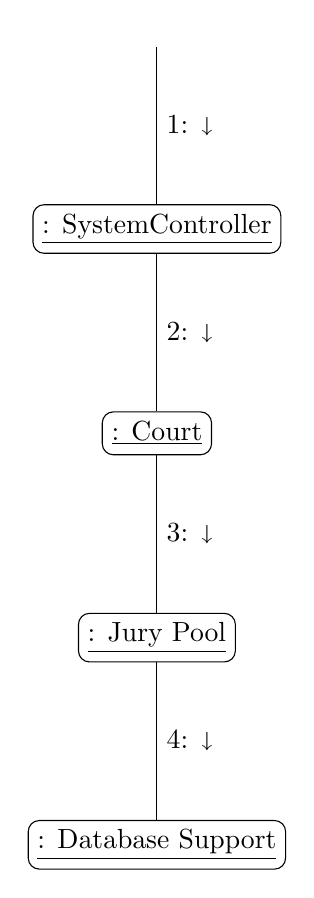
\begin{tikzpicture}[
  auto,
  block/.style = {
    rectangle,
    draw=black,
    align=center,
    rounded corners
  }
]
\node[] (start)  {};
%     style     location                variable name    content 
\node[block, below = 2cm of start]      (controller) {\underline{: SystemController}};
\node[block, below = 2cm of controller]      (court) {\underline{: Court}};
\node[block, below = 2cm of court]      (juryPool) {\underline{: Jury Pool}};
\node[block, below = 2cm of juryPool]      (databaseSupport) {\underline{: Database Support}};

%     (start_node) -- (end_node)   node[location] {content}
\draw (start)      -- (controller) node[midway] {1: $\shortdownarrow$};
\draw (controller) -- (court) node[midway] {2: $\shortdownarrow$};
\draw (court)      -- (juryPool) node[midway] {3: $\shortdownarrow$};
\draw (juryPool)   -- (databaseSupport) node[midway] {4: $\shortdownarrow$};
\end{tikzpicture}

\vspace{0.5cm}

\begin{enumerate}
  \item \texttt{getJurorsInPool():List<Juror>}
  \item \texttt{getJurorsInPool():List<Juror>}
  \item \texttt{getJurorsInPool():List<Juror>}
  \item \texttt{getJurorsInPool():List<Juror>}
\end{enumerate}
\end{center}

\end{document}
